\chapter[Practical Hybrid Quantum-Classical Computing]{Practical Hybrid Quantum-Classical\\Computing} \label{chap:practical-hybrid-quantum-classical-computing}
This chapter is focused on the practical execution of \glspl{hqca} using the Quantum Inspire quantum computing platform and SURF's \gls{hpc} center.
It will start with describing the relevant platforms, followed by reviewing and analyzing how these platforms are used to execute \glspl{hqca} in different workflows.
We will then explore and describe different methods to increase the efficiency of the execution of \glspl{hqca}.

\section{Quantum Inspire}
Quantum Inspire is a full-stack quantum computing platform that QuTech launched last year to make quantum systems available to the general public for exploratory research~\cite{last2020quantum}.
Users can run quantum circuits on different back-ends through the Quantum Inspire web editor or by using the Python \gls{sdk}.
The \gls{cqasm}~\cite{khammassi2018cqasm} is used for describing quantum circuits, but the popular quantum computing frameworks ProjectQ~\cite{steiger2018projectq} and Qiskit~\cite{qiskit} are also supported by the Python \gls{sdk}.
Quantum Inspire supports the execution of quantum circuits on real \glspl{qpu} and through quantum simulation.
An overview of the Quantum Inspire workflow and available device back-ends is shown in \Cref{fig:qi-workflow}.

The two available \glspl{qpu} are Starmon-5 and Spin-2 which have five and two qubits respectively.
These \glspl{qpu} suffer from noise, limited coherence time, limited qubit connectivity, and each \gls{qpu} has a specific allowed gate set.
Note that these gate sets are universal, and non-native gates are decomposed into supported gates depending on the \gls{qpu}.
Regardless of the limitations of these \glspl{qpu}, they are an essential part in research towards better quantum hardware and quantum algorithms.
\begin{figure}[ht]
    \centering
    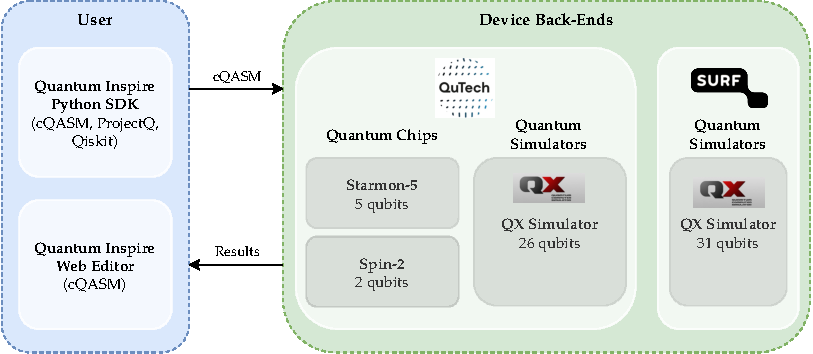
\includegraphics[width=1\linewidth]{figures/qi-workflow.pdf}
    \caption[Overview of the Quantum Inspire workflow.]{
        Overview of the Quantum Inspire workflow.
        Users can submit quantum circuits written in \gls{cqasm} using the web editor or Python \gls{sdk}.
        After the program has been run, the results are returned to the user.
        The quantum circuit can be executed on one of the \glspl{qpu} or simulated using one of the QX simulator back-ends.
        QuTech's simulator back-end supports simulations up to 26 qubits, while SURF's simulator back-end supports simulations up to 35 qubits.
    }
    \label{fig:qi-workflow}
\end{figure}

In the absence of large-scale and fault-tolerant quantum computers, quantum computer simulation is critical for developing and testing quantum algorithms.
Quantum computer simulators often use one of three classical algorithms to simulate quantum circuits.
These algorithms have different trade-offs in the resources that they use.
First, there is the naive Schr{\"o}dinger simulation algorithm in which the complex amplitudes of a quantum state are represented in a state-vector, gates are represented as matrices, and state evolution is done by matrix-vector multiplication.
This algorithm uses $O(2^n)$ time and space, where $n$ is the amount of qubits~\cite{aaronson2016complexity}.
Second, there is the Feynman simulation algorithm which makes use of the path integral formulation of quantum mechanics~\cite{feynman2005space}.
This approach uses $O(m+n)$ space, but takes $O(4^m)$ time, where $m$ is the amount of gates~\cite{aaronson2016complexity}.
So while using a linear amount of space, the time it takes grows exponential with the number of gates.
The number of gates even for small computations can reach the order of thousands.
Supercomputers may be able to simulate quantum circuits with a thousand gates using the Schr{\"o}dinger  algorithm, but not even the most powerful supercomputer could simulate such circuit using the Feynman algorithm.
On the other hand, the Feynman algorithm can simulate a quantum circuit with a few gates and 100 qubits, while the Schr{\"o}dinger algorithm is greatly limited in the amount of qubits it can simulate due to its exponential space requirement.
Finally, \textcite{aaronson2016complexity} described an algorithm that offers best of both worlds: the Schr{\"o}dinger-Feynman algorithm.
This algorithm uses $O(d^n)$ time and $O(d \cdot n \log n)$ space, where $d$ is the depth of the circuit.
These different simulation algorithms allow you to trade time for space efficiency and vice versa, but all of them require exponential time and/or space, greatly limiting the size of simulations we can do.

Quantum Inspire offers two simulator back-ends which use QX~\cite{khammassi2017qx} as quantum computer simulator.
The QX simulator uses the Schr{\"o}dinger simulation algorithm focused on efficiently using sparse operators.
One of the simulator back-ends is hosted by QuTech on a commodity cloud-based server with 4 GB of memory, which can run simulations up to 26 qubits.
The other simulator back-end is hosted on SURF's computer cluster Lisa which consists of several hundreds of multi-core nodes.
The largest node available on Lisa has 1.5 TB of memory, which supports simulations up to 35 qubits.

When quantum circuits are submitted to Quantum Inspire, they are handed to a job scheduler which will attempt to schedule the job as quickly as possible when the requested resources are available.
For the \glspl{qpu} and QuTech simulator back-ends, the jobs are simply placed in a queue which are executed in first-in-first-out order.
The wait time for these back-ends ranges from seconds to minutes.
For the SURF simulator back-end, the jobs are handled by a batch system.
Because SURF's infrastructure is shared with many other users, wait times can vary from minutes to hours.
Especially large simulations which require a large amount of resources may take a long time to schedule.

\section{SURF High Performance Computing}
SURF offers an integrated ICT research infrastructure and provides services in the areas of computing, data storage, visualization, networking, and cloud.
This report is mainly interested in the computing services, and more precisely the Lisa and Cartesius cluster computers.
These cluster computers can be thought of as a network of computers (nodes).
Each node has its own \glspl{cpu}, memory, disk space, and a shared file system.
Cluster computers are often used for \acrfull{hpc}, where a large amount of resources (\glspl{cpu}, \glspl{gpu}, memory, etc.) are used to solve computationally expensive problems.
Interacting with a cluster computer works different than a regular computer: instead of submitting a script or command (job) and immediately being run, cluster computers use a batch system that runs your job as soon as sufficient resources are available.
Lisa and Cartesius use the Slurm workload manager~\cite{yoo2003slurm} as job scheduler.
The specifications of the Lisa and Cartesius cluster computers are described in \Cref{table:surf-cluster-computers}.
\begin{table}[ht]
    \centering
    \begin{tabular}{ c|c|c }
        Resource & Lisa & Cartesius \\
        \hline
        \glspl{cpu} & 5304 & 47,776   \\
        Memory & 41.7 TB & 130 TB \\
        \glspl{gpu} & 216 & 132 \\
        Flop/s (64-bit floating point) & 367.9 Tflop/s & 1.843 Pflop/s  \\
        Disk space & 400 TB home & 180 TB home, 7.7 PB project + scratch \\
    \end{tabular}
    \caption[Specification of the Lisa and Cartesius cluster computers.]{
        Specification of the Lisa and Cartesius cluster computers.
        Here Flop/s refers to floating point operations per second, or the theoretical peak performance.
        Cartesius is the Dutch national supercomputer meant for large computations that require many cores, large symmetric multiprocessing nodes, large amounts of memory, a fast interconnect, large amount of disk space, or a fast I/O subsystem.
        Lisa is meant for tasks that need large computing capacities, but do not need the facilities of a real supercomputer.
    }
    \label{table:surf-cluster-computers}
\end{table}

The Lisa and Cartesius cluster computers consist of login nodes and batch nodes.
One connects to the system through the login node, which is an interactive system similar to a personal computer.
These login nodes can be used for light tasks such as writing and compiling software, writing job scripts, and preparing data.
A job script is essentially a recipe of commands that you want your job job to execute.
Through this script you can load the required modules, handle input and output data processing, define the amount of resources your job requires, and handle the running of the actual application.
The job script is submitted to the job scheduler and will be run on a batch node as soon as the requested resources are available.

\section{Hybrid Quantum-Classical Workflows} \label{sec:workflows}
When researching and running \glspl{hqca}, different problems require different workflows.
For example, small simulation experiments do not require \gls{hpc} facilities, unless one wants to run the experiment many times in parallel with varying parameters.
In \Cref{table:hqca-workflows} the five different workflows which are considered in this report are described.
The order in which the workflows are displayed can be thought of as progressing from small experimentation and prototyping to (large) well-defined experiments.
First, the Local-Local hybrid quantum-classical workflow is often enough for most use cases as most research towards \glspl{hqca} does not require \gls{hpc} facilities or access to a \gls{qpu}.
The Local-\gls{hpc} workflow is useful for large quantum circuit simulations that exceed the resources of modern laptops.
In such case the \gls{hpc}-\gls{hpc} workflow may also be used to reduce network overhead and repeated scheduler wait times.
Generally, one wants the quantum and classical part to be as close to each other as possible, and ideally on the same network.
This is usually possible for quantum simulators, but becomes more difficult when dealing with \glspl{qpu}.
The Local-\gls{qpu} workflow is useful for experimenting and testing out quantum hardware.
In the context of \glspl{hqca}, this can be useful for running small experiments and seeing how noise affects the performance of the algorithm.
For larger and more well-defined experiments, the \gls{hpc}-\gls{qpu} workflow offers the advantage of being able to run experiments unattended.
One could for example define multiple experiments with different parameters and run it over night on SURF's cluster computer.
This is also the biggest advantage of the \gls{hpc}-\gls{hpc} workflow --- one could run many experiments in parallel instead of being limited to local resources.

\begin{table}[ht]
    \centering
    {\renewcommand{\arraystretch}{1.35}
        \begin{tabular}{ c|c|c|>{\centering\arraybackslash}m{4.9cm} }
            Workflow name & Classical part & Quantum part & Use case(s) \\
            \hline
            Local-Local & Local & Simulation (Local) & Small experimentation/prototyping \\
            \hline
            Local-\gls{hpc} & Local & Simulation (\gls{hpc}) & Large quantum simulations that can not be run locally \\
            \hline
            Local-\gls{qpu} & Local & \gls{qpu} & Small experimentation/exploration of hardware \\
            \hline
            \gls{hpc}-\gls{qpu} & \gls{hpc} & \gls{qpu} & Well-defined/multiple experiments, hybrid computation with expensive classical part \\
            \hline
            \gls{hpc}-\gls{hpc} & \gls{hpc} & Simulation (\gls{hpc}) & Multiple experiments, expensive classical and/or quantum part, high performance simulations \\
        \end{tabular}
    }
    \caption[Relevant hybrid quantum-classical workflows and their use cases.]{
        Relevant hybrid quantum-classical workflows and their use cases.
        In the classical part column the platform on which the classical computation runs: locally on a laptop or personal computer, or on SURF's \gls{hpc} center.
        Equivalently, the quantum part columns refers to the platform the quantum computation runs on: local simulation, \gls{qpu}, or simulation on SURF's \gls{hpc} center.
    }
    \label{table:hqca-workflows}
\end{table}
% mostly research towards HQCA's, not really practical applications/no speedups to be gained yet
% most research towards HQCA's doesnt need supercomputers - can still be useful for running multiple experiments

\section{Hybrid Quantum-Classical Workflow Analysis} \label{sec:hqca-analysis}
In this section we define and analyze the efficiency of executing \glspl{hqca} using the different workflows defined in the previous section.
There are many variables to be considered when talking about the efficiency of a hybrid quantum-classical workflow: network latency, circuit optimization, scheduler wait times, optimizer choice, etc.
In the end, the aim is to reduce the amount of time it takes to run a full experiment.
The variables we consider to describe the efficiency of a hybrid quantum-classical experiment in this report are as follows:
\begin{itemize}
    \item $T_Q(n, d, s)$ describes the quantum circuit execution time where $n$ is the number of qubits, $d$ the depth of the quantum circuit, and $s$ the number of shots.
    \item $T_L$ describes the latency between the classical and quantum computation. This includes latencies such as network overhead, scheduler wait time, resource initialization, etc.
    \item $T_C(p)$ describes the time taken by the classical optimization algorithm for $p$ parameters.
\end{itemize}
The efficiency of a hybrid quantum-classical experiment is then defined by the sum of these variables:
\begin{equation}
T_\text{total} = T_Q(n, d, s) + T_L + T_C(p),
\end{equation}
and a lower value is considered more efficient.

To get an initial understanding on the efficiency of different quantum back-ends we implement and benchmark the \gls{qaoa} to solve the \gls{maxcut} problem on a 2-regular graph with 4 vertices (qubits) and edges.
The details of the \gls{maxcut} problem and the \gls{qaoa} implementation are described in \Cref{chap:qaoa-maxcut}.
This report will mainly focus on the quantities $T_Q$ and $T_L$ as they are the largest and most relevant.
Some work related to optimizing the classical optimization part has been done by \textcite{lavrijsen2020classical} and \textcite{sung2020exploration}.
The benchmark results are displayed in \Cref{table:baseline-benchmark}.
The efficiency of these different quantum parts should not be compared to each other as each quantum part is a different tool with a different application.
Rather, it can be interpreted as a demonstration of how different quantum parts behave on the same problem.

\begin{table}[ht]
    \centering
    {\renewcommand{\arraystretch}{1.35}
        \begin{tabular}{ c|c|c|c }
            Quantum part & $T_Q(n, d, s)$ & $T_L$ & $T_Q(n, d, s) + T_L$ \\
            \hline
            Simulation (Local, Qiskit) & $0.009\text{s} \pm 0.001$s & $0.010 \text{s} \pm 0.022$s & $0.019 \text{s} \pm 0.023$s \\
            Simulation (\gls{hpc}) & $0.016\text{s} \pm 0.001$s & $11.734\text{s} \pm 2.029$s & $11.751\text{s} \pm 2.029$s \\
            \gls{qpu} (Starmon-5) & $0.622\text{s} \pm 0.000$s & $27.742\text{s} \pm 0.610$s & $28.365\text{s} \pm 0.610$s \\
        \end{tabular}
    }
    \caption[Benchmarks of the time taken by different quantum parts in the context of a hybrid quantum-classical computation.]{
        Benchmarks of the time taken by different quantum parts in the context of a hybrid quantum-classical computation.
        We measure the quantum execution time $T_Q(n, d, s)$ and latency $T_L$ for 150 quantum circuit executions for every quantum part, with $n = 4$, $d = 32$, and $s = 4096$.
        The values shown are the mean and standard deviation of the 150 runs.
    }
    \label{table:baseline-benchmark}
\end{table}

Given the measurements from \Cref{table:baseline-benchmark}, we can estimate how much time it would take to execute a meaningful and practical \gls{hqca} experiment.
In the context of running the \gls{vqe} on a hardware back-end, \textcite{kandala2017hardware} estimate that with the current architecture in the order of $10^5$ (best case) to $10^6$ (worst case) quantum circuit executions are needed to achieve results within chemical accuracy.
This is a very rough estimate, as the amount of circuit executions required depends on the problem at hand, desired accuracy, hardware error rates, choice of ansatz, etc.
Using the total average time taken per circuit execution by the Starmon-5 \gls{qpu} from \Cref{table:baseline-benchmark}, this would take in the order of 32 to 328 days just in quantum execution and wait time.
On top of that, there is an additional development time that should be considered, which includes debugging and testing quantum circuit behavior using quantum circuit simulators.
In the following sections we will explore different methods of potentially increasing the efficiency of the execution of \glspl{hqca}.

\subsection{Development Cycle}
The development cycle of \glspl{hqca} usually consists of three phases of quantum circuit execution: noiseless simulation, noisy simulation, and hardware.
Quantum Inspire's \gls{qpu} and simulation back-ends are all in the cloud, introducing a network overhead.
While this is hard to avoid for the \gls{qpu} back-ends, for some applications of the simulator back-ends this network overhead may be avoided through local simulation.
This is especially true for simulations of approximately 24 qubits and lower, for which the benefits of \gls{hpc} do not yet become substantial.
For this range of simulations, the network and possible job queue overhead greatly exceeds the actual quantum circuit execution time.
To avoid this unnecessary overhead for small simulations, support for a local simulation back-end in Quantum Inspire can be useful.
As per the measurements from \Cref{table:baseline-benchmark}, local simulation is a factor of $\sim1000$ faster for 4-qubit simulations over \gls{hpc} simulation because of the network and job scheduler overhead.

Another way to increase the efficiency of the \gls{hqca} development cycle is to reduce the amount of circuits that need to be executed on a \gls{qpu}.
This can be achieved if one has access to a noisy quantum simulator which models the target \gls{qpu}'s hardware noise well.
QX simulator supports the quantum depolarizing channel~\cite[Section 8.3.4]{nielsen2002quantum}, which is a standard model for noise in quantum systems.
However, the quantum depolarizing channel does not accurately represent the errors encountered on actual \glspl{qpu}.
By adding support for better user-configurable error channels that correspond more to actual hardware noise, the amount of quantum circuits that need to be executed on actual \glspl{qpu} can be decreased.
One can then use the noisy quantum simulator for a larger part of the development process, which will increase the development efficiency as quantum circuit simulation is often more accessible and has less overhead cost.

\subsection{QX Simulator Batch Parameters}
When submitting a job to the job scheduler on SURF's \gls{hpc} center, one can define the resources required for the job through batch parameters.
Choosing the right parameters for a job can optimize its execution time and help the job scheduler use the system's resources as optimal as possible.
In the context of the SURF QX simulator back-end, we are interested in figuring out the optimal amount of cores and memory to use for quantum circuit simulations of different qubit counts.
Choosing the optimal amount of cores improves both the quantum simulation execution time ($T_Q$) and scheduling efficiency ($T_L$), whereas choosing the right amount of memory ensures that the simulation has access to enough memory and increases scheduling efficiency.
We run all experiments and benchmarks on SURF's cluster computer Lisa on the quantum computing nodes (\mintinline{bash}{fat_soil_shared} partition).
This partition consists of four nodes with 1.5 TB memory, two NVIDIA TitanRTX \glspl{gpu}, and four sockets with 10 \glspl{cpu} per socket.
These quantum nodes are especially tailored for the development and execution of (hybrid) quantum simulations.

\subsubsection{Number of Cores Parameter}
To determine the optimal amount of cores to use for a given number of qubits, we measured the execution time of QX simulator for quantum circuits with different number of qubits.
The quantum circuits used are circuits generated by our \gls{qaoa} implementation on the \gls{maxcut} problem.
For each number of qubits $n$, we generate a \gls{qaoa} \gls{maxcut} circuit on a random 2-regular graph with $n$ vertices.
These random graphs are generated with no self-loops or parallel edges according to the algorithm described by \textcite{steger1999generating}.
The respective quantum circuit for a 2-regular graph with $n$ vertices has a depth $d$ of $4n$.
This means that the depth increases as the number of qubits and problem size increases, as is the case with most realistic implementations of quantum algorithms.
The thread affinity was set up in a way that the threads run as much on the same \gls{cpu} socket(s) as possible according to the layout from \Cref{table:fat-soil-affinities}.
\begin{table}[ht]
    \centering
    {\renewcommand{\arraystretch}{1.15}
        \begin{tabular}{c|c}
            \gls{cpu} socket & \glspl{cpu} \\
            \hline
            0 & 0, 4, 8, 12, 16, 20, 24, 28, 32, 36 \\
            1 & 1, 5, 9, 13, 17, 21, 25, 29, 33, 37 \\
            2 & 2, 6, 10, 14, 18, 22, 26, 30, 34, 38 \\
            3 & 3, 7, 11, 15, 19, 23, 27, 31, 35, 39 \\
        \end{tabular}
    }
    \caption[Overview of the layout of the sockets and \glspl{cpu} on the \mintinline{bash}{fat_soil_shared} quantum nodes.]{
        Overview of the layout of the sockets and \glspl{cpu} on the \mintinline{bash}{fat_soil_shared} quantum nodes.
        Each node has 4 sockets with 10 \glspl{cpu} per socket for a total of 40 \glspl{cpu}.
    }
    \label{table:fat-soil-affinities}
\end{table}

The benchmark results are displayed in \Cref{table:qx-benchmark}.
For lower qubit counts adding more cores does not or only slightly improve the execution time.
Given the limited amount of resources available on the quantum nodes and the minor speedup gained, simulations below 20 qubits should probably not be given more than one or two cores.
For simulations of 20 qubits and above, increasing the amount of cores becomes more fruitful.
As the number of qubit increases, the execution time increases exponentially, and for simulations of 20 qubits and more, increasing the amount of cores begins to save time in the order of seconds and even minutes.
These higher qubit simulations can be sped up an order of 7 to 10 by using 32 or more cores.
The speedup stagnates greatly after 32 cores, and while for some cases the speedup continues to increase beyond 32 cores, it is a relatively small speedup.
Depending on the seasonality, 32 cores per simulation might occupy too many resources.
In this case, a speedup on the order of 4 to 5 may still be achieved with 16 cores.
The trade-off to be considered when choosing the amount of cores to use per number of qubits depends on the available resources, seasonality, and speedup gained.
The performance of quantum circuit simulation can be further pushed by using \glspl{gpu} as shown in \cite[Appendix B]{oud2019simulation}, however QX simulator does not currently support \gls{gpu} simulation.

\clearpage

\begin{sidewaystable}
    \centering
    {\renewcommand{\arraystretch}{1.15}
        \setlength{\tabcolsep}{2.5pt}
        \begin{tabular}{ccccccccccccc}
            $n$ & $d$ & $t = 1$ & $t = 2$ & $t = 4$ & $t = 8$ & $t = 16$ & $t = 20$ & $t = 24$ & $t = 28$ & $t = 32$ & $t = 36$ & $t = 40$ \\
            \hline
            $4$ & $16$ & $0.026$s & \underline{$\mathbf{0.023}$\textbf{s}} & $0.027$s & $0.027$s & $0.027$s & $0.025$s & $0.027$s & $0.031$s & $0.031$s & $0.032$s & $0.043$s \\
            $6$ & $24$ & $0.023$s & $0.024$s & \underline{$\mathbf{0.023}$\textbf{s}} & $0.027$s & $0.028$s & $0.028$s & $0.028$s & $0.032$s & $0.032$s & $0.028$s & $0.031$s \\
            $8$ & $32$ & \underline{$\mathbf{0.023}$\textbf{s}} & $0.025$s & $0.025$s & $0.028$s & $0.028$s & $0.025$s & $0.027$s & $0.031$s & $0.030$s & $0.028$s & $0.035$s \\
            $10$ & $40$ & \underline{$\mathbf{0.023}$\textbf{s}} & $0.024$s & $0.026$s & $0.025$s & $0.030$s & $0.030$s & $0.028$s & $0.028$s & $0.028$s & $0.027$s & $0.041$s \\
            $12$ & $48$ & $0.025$s & $0.026$s & \underline{$\mathbf{0.023}$\textbf{s}} & $0.028$s & $0.029$s & $0.035$s & $0.029$s & $0.027$s & $0.034$s & $0.029$s & $0.045$s \\
            $14$ & $56$ & $0.032$s & $0.032$s & \underline{$\mathbf{0.027}$\textbf{s}} & $0.030$s & $0.030$s & $0.032$s & $0.028$s & $0.033$s & $0.027$s & $0.029$s & $0.044$s \\
            $16$ & $64$ & $0.047$s & $0.041$s & $0.041$s & $0.039$s & \underline{$\mathbf{0.028}$\textbf{s}} & $0.042$s & $0.039$s & $0.038$s & $0.030$s & $0.038$s & $0.042$s \\
            $18$ & $72$ & $0.106$s & $0.070$s & $0.053$s & $0.051$s & $0.050$s & $0.039$s & $0.049$s & \underline{$\mathbf{0.037}$\textbf{s}} & $0.039$s & $0.042$s & $0.043$s \\
            $20$ & $80$ & $0.417$s & $0.242$s & $0.145$s & $0.105$s & $0.078$s & $0.072$s & $0.083$s & $0.085$s & \underline{$\mathbf{0.069}$\textbf{s}} & $0.075$s & $0.075$s \\
            $22$ & $88$ & $2.023$s & $1.102$s & $0.719$s & $0.553$s & $0.353$s & $0.292$s & $0.264$s & $0.234$s & $0.219$s & $0.213$s & \underline{$\mathbf{0.213}$\textbf{s}} \\
            $24$ & $96$ & $8.853$s & $4.800$s & $3.164$s & $2.533$s & $1.685$s & $1.446$s & $1.297$s & $1.187$s & $1.087$s & $1.026$s & \underline{$\mathbf{0.983}$\textbf{s}} \\
            $26$ & $104$ & $38.943$s & $20.991$s & $13.787$s & $11.045$s & $7.390$s & $6.668$s & $5.734$s & $5.212$s & $4.805$s & $4.512$s & \underline{$\mathbf{4.318}$\textbf{s}} \\
            $28$ & $112$ & $165.9$s & $89.2$s & $58.5$s & $46.9$s & $36.2$s & $36.2$s & $33.2$s & $28.9$s & $24.9$s & \underline{$\mathbf{22.7}$\textbf{s}} & $27.4$s \\
            $30$ & $120$ & $709$s & $380$s & $249.1$s & $199.5$s & $157.2$s & $139.5$s & $117.3$s & $112.2$s & \underline{$\mathbf{102.2}$\textbf{s}} & $106.8$s & $104.8$s \\
            $31$ & $124$ & $1472.5$s & $790.6$s & $516.8$s & $414$s & $290.8$s & $273.1$s & $240.1$s & $223.2$s & $211.4$s & \underline{$\mathbf{206.1}$\textbf{s}} & $207.2$s \\
            $32$ & $128$ & $3057.3$s & $1632.7$s & $1063.3$s & $848.4$s & $589.4$s & $521.4$s & $463.4$s & $422$s & $393.5$s & $375.7$s & \underline{$\mathbf{358.2}$\textbf{s}} \\
            $33$ & $132$ & $6307.4$s & $3394.2$s & $2206.7$s & $1770.6$s & $1198.8$s & $1090.5$s & $1030.3$s & $1114.8$s & $898.1$s & $883.2$s & \underline{$\mathbf{837}$\textbf{s}} \\
            $34$ & $136$ & $14827.4$s & $7855.2$s & $4996.7$s & $3853.7$s & $2325.1$s & $2066.3$s & $1798.9$s & $2043.4$s & $1498.6$s & $1454.3$s & \underline{$\mathbf{1390.7}$\textbf{s}} \\
            $35$ & $140$ & $37658.7$s & $20438.4$s & $12516.8$s & $9242.1$s & $4926.8$s & $4034.7$s & $3424.5$s & $4063.6$s & $2936.7$s & $2769.5$s & \underline{$\mathbf{2679}$\textbf{s}} \\
        \end{tabular}
    }
    \caption[Benchmark results of the execution time of quantum circuits using QX simulator for different qubit and core counts.]{
        Benchmark results of the execution time of quantum circuits using QX simulator for different qubit and core counts.
        Here $n$ is the number of qubits, $d$ is the depth of the circuit, and $t$ is the number of cores.
        Execution times shown are the average of 10 repeated circuit executions.
        The optimal amount of cores $t$ is highlighted for every $n$.
    }
    \label{table:qx-benchmark}
\end{sidewaystable}

\clearpage

\subsubsection{Memory Parameter}
The \mintinline{bash}{fat_soil_shared} partition is composed of shared nodes, which means that multiple users can run jobs on the same node and resources like memory and disk space are shared.
For this reason, to ensure that a simulation has access to enough memory, the simulation job should specify the amount of memory it needs.
By default, a job on the \mintinline{bash}{fat_soil_shared} partition is given $37.5$ GB of memory per requested core.
This is not a fit default for QX simulator, as its memory usage grows with the number of qubits, not necessarily the amount of cores it uses.
To ensure that simulations request a reasonable amount of memory, we measure the memory usage of QX simulator running random circuits of depth 2 for different number of qubits.
This is done by spawning a QX simulator process and polling the operating system every 0.1 millisecond for the respective process' \gls{rss} memory usage.
We then take the highest amount of memory measured by polling and take that as the ``total" memory usage of the simulation.
This is repeated 10 times per $n$ qubits.
The results are displayed in \Cref{table:qx-memory-usage}.
We plot the data in \Cref{fig:qx-memory-plot}, along with a fitted exponential function to predict the amount of memory $\hat{m}$ required (in GB) for a simulation of $n$ qubits:
\begin{equation}
\hat{m}(n) = \left(3.20017417 \cdot 10^{-8}\right) \cdot e^{0.693145626n} + 0.0210389214.
\end{equation}
This function is especially useful to define the memory requirement for simulations of $n \ge 31$ qubits, where the default of $37.5$ GB of memory per requested core becomes too small.

\begin{table}[H]
    \centering
    \begin{tabular}{cc}
        $n$ & \gls{rss} memory usage \\
        \hline
        1 & $\text{18.96 MB} \pm \text{918.08 kB}$ \\
        2 & $\text{19.72 MB} \pm \text{1.80 MB}$ \\
        3 & $\text{19.97 MB} \pm \text{971.35 kB}$ \\
        4 & $\text{19.72 MB} \pm \text{1.13 MB}$ \\
        5 & $\text{20.28 MB} \pm \text{1.68 MB}$ \\
        6 & $\text{19.52 MB} \pm \text{1.04 MB}$ \\
        7 & $\text{20.74 MB} \pm \text{2.19 MB}$ \\
        8 & $\text{19.89 MB} \pm \text{1.53 MB}$ \\
        9 & $\text{19.79 MB} \pm \text{1.12 MB}$ \\
        10 & $\text{19.87 MB} \pm \text{991.81 kB}$ \\
        11 & $\text{19.45 MB} \pm \text{1.03 MB}$ \\
        12 & $\text{19.48 MB} \pm \text{1.24 MB}$ \\
        13 & $\text{20.00 MB} \pm \text{1.93 MB}$ \\
        14 & $\text{19.64 MB} \pm \text{1.02 MB}$ \\
        15 & $\text{20.77 MB} \pm \text{725.03 kB}$ \\
        16 & $\text{23.35 MB} \pm \text{2.19 MB}$ \\
        17 & $\text{21.51 MB} \pm \text{935.23 kB}$ \\
        18 & $\text{26.94 MB} \pm \text{1.46 MB}$ \\
    \end{tabular}
    \quad
    \begin{tabular}{cc}
        $n$ & \gls{rss} memory usage \\
        \hline
        19 & $\text{36.45 MB} \pm \text{715.73 kB}$ \\
        20 & $\text{53.87 MB} \pm \text{915.52 kB}$ \\
        21 & $\text{88.12 MB} \pm \text{159.36 kB}$ \\
        22 & $\text{153.70 MB} \pm \text{1.63 MB}$ \\
        23 & $\text{288.00 MB} \pm \text{858.89 kB}$ \\
        24 & $\text{555.85 MB} \pm \text{742.69 kB}$ \\
        25 & $\text{1.09 GB} \pm \text{2.47 MB}$ \\
        26 & $\text{2.17 GB} \pm \text{892.79 kB}$ \\
        27 & $\text{4.32 GB} \pm \text{963.74 kB}$ \\
        28 & $\text{8.61 GB} \pm \text{1.02 MB}$ \\
        29 & $\text{17.20 GB} \pm \text{1.28 MB}$ \\
        30 & $\text{34.38 GB} \pm \text{2.26 MB}$ \\
        31 & $\text{68.74 GB} \pm \text{781.89 kB}$ \\
        32 & $\text{137.46 GB} \pm \text{1.05 MB}$ \\
        33 & $\text{274.90 GB} \pm \text{901.16 kB}$ \\
        34 & $\text{549.78 GB} \pm \text{1.17 MB}$ \\
        35 & $\text{1.10 TB} \pm \text{995.41 kB}$ \\
        \phantom{36} & \\
    \end{tabular}
    \caption[QX simulator \gls{rss} memory usage for varying number of qubits.]{
        QX simulator \gls{rss} memory usage for varying number of qubits.
        The measurements shown are the average taken of 10 runs.
    }
    \label{table:qx-memory-usage}
\end{table}

\begin{figure}[ht]
    \centering
    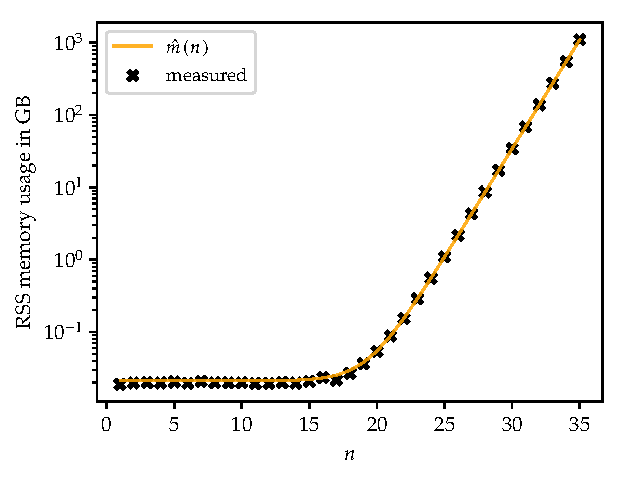
\includegraphics[width=0.765\linewidth]{figures/qx_memory_plot.pdf}
    
    \caption[Plot of the \gls{rss} memory usage of QX simulator as the number of qubits increases.]{
        Plot of the \gls{rss} memory usage of QX simulator as the number of qubits increases.
        We use non-linear least squares~\cite{branch1999subspace} to fit an exponential function $\hat{m}(n) = a \cdot e^{bn} + c$ to the data, which gives $a = 3.20017417 \cdot 10^{-8}$, $b = 0.693145626$, and $c = 0.0210389214$ with $R^2 = 0.99$.
        We fit the function to the mean of 10 runs plus its standard deviation to err on the high side to ensure that the simulation has more than enough memory available.
    }
    \label{fig:qx-memory-plot}
\end{figure}

\subsection{Parallel Quantum Circuit Execution}
In the \gls{vqe} one uses a quantum computer to measure the energy of a molecular Hamiltonian.
As described in \Cref{sec:vqe}, this is done by decomposing the Hamiltonian into a linear combination of Pauli operators~(\Cref{eq:pauli_hamiltonian}).
Consider the following simple one-qubit Hamiltonian:
\begin{equation}
H = g_0Z_0 + g_1X_0,
\end{equation}
for which the energy is given as
\begin{equation}
\expval{H} = g_0\expval{Z_0} + g_1\expval{X_0},
\end{equation}
where $g_0$ and $g_1$ are some constants.
Since the Pauli terms $\expval{Z_0}$ and $\expval{X_0}$ do not commute and measurement is destructive, we need to run the same quantum circuit twice: once for measuring $\expval{Z_0}$, and once for measuring $\expval{X_0}$.
These circuit evaluations are independent of each other and could be executed in parallel to cut the calculation time in half.
The number of measurement directions required per energy measurement increases rapidly for molecular Hamiltonians: the LiH and $\ensuremath{\mathrm{BeH_2}}$ molecules require 25 and 44 measurement directions respectively~\cite[Supplementary Information, Section III]{kandala2017hardware}.
For simulator back-ends this parallelization is easily achieved by simply running multiple simulations in parallel.
Even more, because we have full access to the state vector in quantum simulation, one can simply save the final state vector of the quantum circuit before measurement and measure in any number of ways you like.
For \gls{qpu} back-ends, this kind of parallelization requires access to multiple \glspl{qpu}.
At this moment, most development in quantum hardware is focused on the quality, and not the quantity of \glspl{qpu}.
However, access to multiple \gls{nisq} devices may be required to make the execution of \glspl{hqca} feasible and practical.
Assuming even access to two \glspl{qpu}, the estimate of the execution time of a meaningful \gls{hqca} experiment given in \Cref{sec:hqca-analysis} can be approximately halved from ranging from 32 to 328 days, to ranging from 16 to 164 days.

\subsection{Quantum Circuit Batching}
\subsubsection{Gradient Circuits Batching}
\subsubsection{Breadth Optimization}